\documentclass[tikz,border=5pt]{standalone}
\usepackage{amsmath}
\usetikzlibrary{arrows.meta,calc}
\tikzset{edge/.style={black!75,thick},electrode/.style={orange!70!black,line width=2.4pt},
vec/.style={-{Stealth[length=2.2mm]},thick},dim/.style={thin},
matone/.style={fill=blue!12},mattwo/.style={fill=orange!13}}
\newcommand{\checker}[4]{%
  \fill[matone] (0,1.65) rectangle (1.65,3.3);
  \fill[matone] (1.65,0) rectangle (3.3,1.65);
  \fill[mattwo] (0,0) rectangle (1.65,1.65);
  \fill[mattwo] (1.65,1.65) rectangle (3.3,3.3);
  \draw[edge] (0,0) rectangle (3.3,3.3);
  \draw[thin] (1.65,0)--(1.65,3.3) (0,1.65)--(3.3,1.65);
  \node at (.825,2.475) {$#1$};\node at (2.475,2.475) {$#2$};
  \node at (.825,.825) {$#3$};\node at (2.475,.825) {$#4$};
}
\begin{document}
% statement-05: a genuinely thin 3D plate; rear/front narrow faces are contacts.
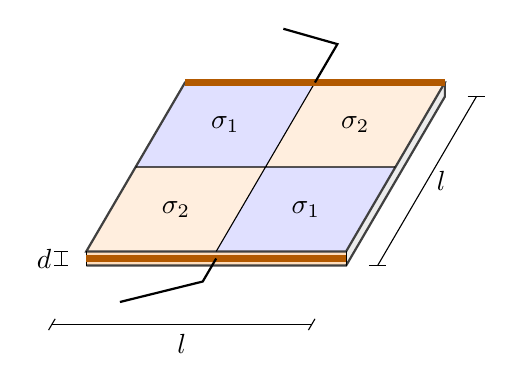
\begin{tikzpicture}[x={(1cm,0cm)},y={(.38cm,.65cm)},z={(0cm,1cm)}]
\fill[orange!26] (0,0,-.18)--(3.3,0,-.18)--(3.3,0,0)--(0,0,0)--cycle;
\fill[gray!15] (3.3,0,-.18)--(3.3,3.3,-.18)--(3.3,3.3,0)--(3.3,0,0)--cycle;
\fill[matone] (0,1.65,0)--(1.65,1.65,0)--(1.65,3.3,0)--(0,3.3,0)--cycle;
\fill[matone] (1.65,0,0)--(3.3,0,0)--(3.3,1.65,0)--(1.65,1.65,0)--cycle;
\fill[mattwo] (0,0,0)--(1.65,0,0)--(1.65,1.65,0)--(0,1.65,0)--cycle;
\fill[mattwo] (1.65,1.65,0)--(3.3,1.65,0)--(3.3,3.3,0)--(1.65,3.3,0)--cycle;
\draw[edge] (0,0,0)--(3.3,0,0)--(3.3,3.3,0)--(0,3.3,0)--cycle;
\draw[thin] (0,1.65,0)--(3.3,1.65,0) (1.65,0,0)--(1.65,3.3,0);
\draw[edge] (0,0,-.18)--(3.3,0,-.18)--(3.3,3.3,-.18)--(3.3,3.3,0);
\draw[thin] (0,0,-.18)--(0,0,0) (3.3,0,-.18)--(3.3,0,0);
\draw[electrode] (0,0,-.09)--(3.3,0,-.09);
\draw[electrode] (0,3.3,0)--(3.3,3.3,0);
\draw[thick] (1.65,3.3,0)--(1.65,4.05,0)--(.85,4.35,0);
\draw[thick] (1.65,0,-.09)--(1.65,-.45,-.09)--(.75,-.85,-.09);
\node at (.825,2.475,0) {$\sigma_1$};\node at (2.475,2.475,0) {$\sigma_2$};
\node at (.825,.825,0) {$\sigma_2$};\node at (2.475,.825,0) {$\sigma_1$};
\draw[dim] (0,-1.15,-.18)--(3.3,-1.15,-.18);
\draw[dim] (0,-1.04,-.18)--(0,-1.26,-.18) (3.3,-1.04,-.18)--(3.3,-1.26,-.18);
\node[below] at (1.65,-1.15,-.18) {$l$};
\draw[dim] (3.7,0,-.18)--(3.7,3.3,-.18);
\draw[dim] (3.59,0,-.18)--(3.81,0,-.18) (3.59,3.3,-.18)--(3.81,3.3,-.18);
\node[right] at (3.7,1.65,-.18) {$l$};
\draw[dim] (-.32,0,-.18)--(-.32,0,0);
\draw[dim] (-.41,0,-.18)--(-.23,0,-.18) (-.41,0,0)--(-.23,0,0);
\node[left] at (-.32,0,-.09) {$d$};
\end{tikzpicture}

% layout-05: u is voltage, psi is a stream function in amperes.
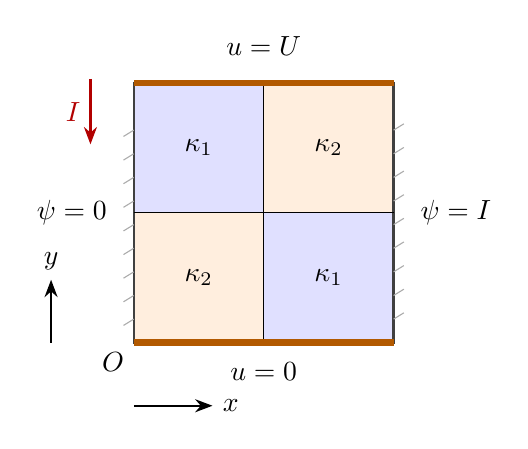
\begin{tikzpicture}
\checker{\kappa_1}{\kappa_2}{\kappa_2}{\kappa_1}
\draw[electrode] (0,3.3)--(3.3,3.3) (0,0)--(3.3,0);
\foreach \v in {.3,.6,...,3.0}{
 \draw[gray!65,thin] (-.13,\v-.08)--(0,\v);
 \draw[gray!65,thin] (3.3,\v)--(3.43,\v+.08);
}
\node[above] at (1.65,3.52) {$u=U$};
\node[below] at (1.65,-.13) {$u=0$};
\node[left] at (-.22,1.65) {$\psi=0$};
\node[right] at (3.52,1.65) {$\psi=I$};
\draw[vec,red!70!black] (-.55,3.35)--(-.55,2.52) node[midway,left] {$I$};
\draw[vec] (0,-.8)--(1.0,-.8) node[right] {$x$};
\draw[vec] (-1.05,0)--(-1.05,.8) node[above] {$y$};
\node[below left] at (0,0) {$O$};
\end{tikzpicture}

% bounds-05: the newly introduced horizontal short and vertical crack differ.
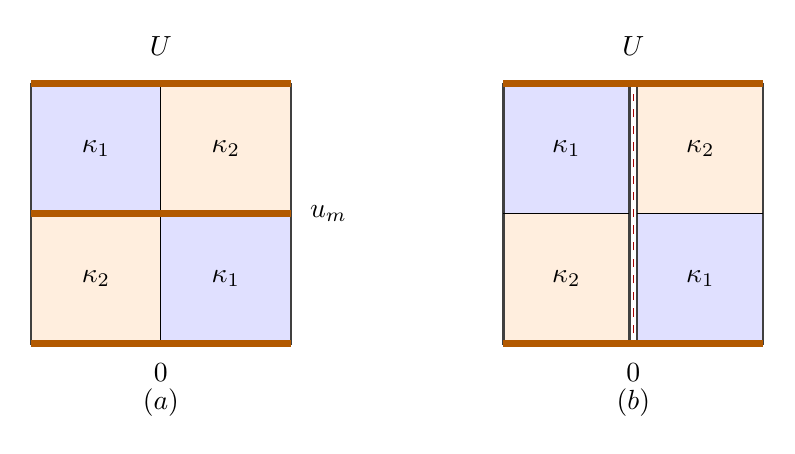
\begin{tikzpicture}
\begin{scope}
\checker{\kappa_1}{\kappa_2}{\kappa_2}{\kappa_1}
\draw[electrode] (0,0)--(3.3,0) (0,3.3)--(3.3,3.3);
\draw[electrode] (0,1.65)--(3.3,1.65);
\node[right] at (3.42,1.65) {$u_m$};
\node[above] at (1.65,3.53) {$U$};\node[below] at (1.65,-.13) {$0$};
\node at (1.65,-.75) {$(a)$};
\end{scope}
\begin{scope}[xshift=6.0cm]
\fill[matone] (0,1.65) rectangle (1.60,3.3);
\fill[mattwo] (0,0) rectangle (1.60,1.65);
\fill[mattwo] (1.70,1.65) rectangle (3.3,3.3);
\fill[matone] (1.70,0) rectangle (3.3,1.65);
\draw[edge] (0,0) rectangle (1.60,3.3) (1.70,0) rectangle (3.3,3.3);
\draw[thin] (0,1.65)--(1.60,1.65) (1.70,1.65)--(3.3,1.65);
\draw[electrode] (0,0)--(3.3,0) (0,3.3)--(3.3,3.3);
\draw[red!65!black,dashed] (1.65,.13)--(1.65,3.17);
\node at (.80,2.475) {$\kappa_1$};\node at (2.50,2.475) {$\kappa_2$};
\node at (.80,.825) {$\kappa_2$};\node at (2.50,.825) {$\kappa_1$};
\node[above] at (1.65,3.53) {$U$};\node[below] at (1.65,-.13) {$0$};
\node at (1.65,-.75) {$(b)$};
\end{scope}
\end{tikzpicture}

% interface-05: an incoming ray with tan(theta1)=2, outgoing tan(theta2)=1/2.
% This local example represents kappa1/kappa2=4, not a global exact streamline.
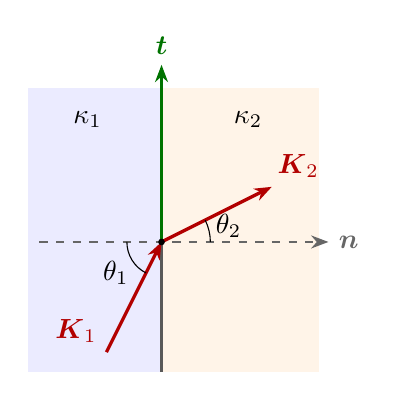
\begin{tikzpicture}
\fill[blue!8] (-1.7,-1.65) rectangle (0,1.95);
\fill[orange!9] (0,-1.65) rectangle (2.0,1.95);
\draw[black!65,thick] (0,-1.65)--(0,2.16);
\draw[vec,dashed,black!60] (-1.55,0)--(2.12,0) node[right] {$\boldsymbol n$};
\draw[vec,green!45!black] (0,0)--(0,2.25) node[above] {$\boldsymbol t$};
\draw[vec,red!70!black,very thick] (-.7,-1.4)--(0,0);
\draw[vec,red!70!black,very thick] (0,0)--(1.4,.7);
\node[left,red!70!black] at (-.7,-1.13) {$\boldsymbol K_1$};
\node[above right,red!70!black] at (1.35,.69) {$\boldsymbol K_2$};
\node at (-.94,1.55) {$\kappa_1$};\node at (1.1,1.55) {$\kappa_2$};
\draw[thin] (-.44,0) arc[start angle=180,end angle=243.435,radius=.44];
\node at (-.58,-.39) {$\theta_1$};
\draw[thin] (.62,0) arc[start angle=0,end angle=26.565,radius=.62];
\node at (.85,.20) {$\theta_2$};
\fill (0,0) circle[radius=1.2pt];
\end{tikzpicture}

% duality-05: simultaneous exchange of phases and Dirichlet/Neumann sides.
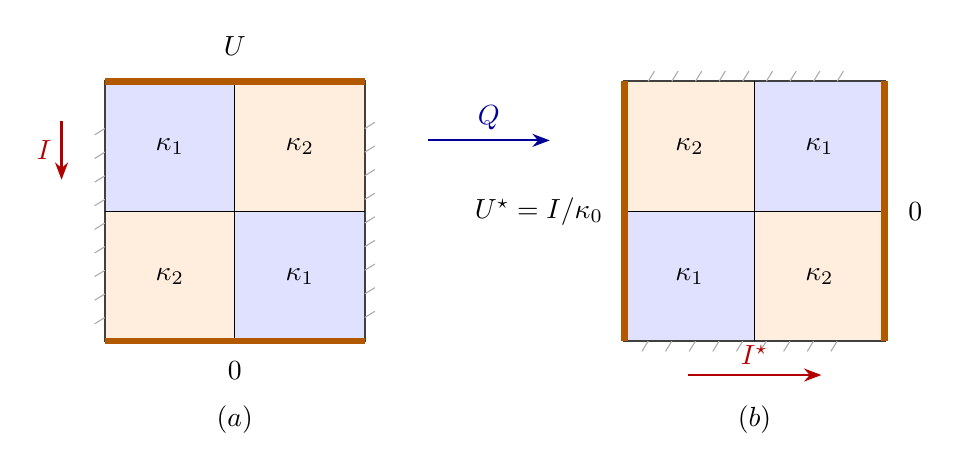
\begin{tikzpicture}
\begin{scope}
\checker{\kappa_1}{\kappa_2}{\kappa_2}{\kappa_1}
\draw[electrode] (0,0)--(3.3,0) (0,3.3)--(3.3,3.3);
\foreach \v in {.3,.6,...,3.0}{
 \draw[gray!65,thin] (-.13,\v-.08)--(0,\v);
 \draw[gray!65,thin] (3.3,\v)--(3.43,\v+.08);
}
\node[above] at (1.65,3.50) {$U$};\node[below] at (1.65,-.13) {$0$};
\draw[vec,red!70!black] (-.55,2.8)--(-.55,2.05) node[midway,left] {$I$};
\node at (1.65,-1.0) {$(a)$};
\end{scope}
\draw[vec,blue!60!black] (4.10,2.55)--(5.65,2.55) node[midway,above] {$Q$};
\begin{scope}[xshift=6.6cm]
\fill[mattwo] (0,1.65) rectangle (1.65,3.3);
\fill[mattwo] (1.65,0) rectangle (3.3,1.65);
\fill[matone] (0,0) rectangle (1.65,1.65);
\fill[matone] (1.65,1.65) rectangle (3.3,3.3);
\draw[edge] (0,0) rectangle (3.3,3.3);
\draw[thin] (1.65,0)--(1.65,3.3) (0,1.65)--(3.3,1.65);
\node at (.825,2.475) {$\kappa_2$};\node at (2.475,2.475) {$\kappa_1$};
\node at (.825,.825) {$\kappa_1$};\node at (2.475,.825) {$\kappa_2$};
\draw[electrode] (0,0)--(0,3.3) (3.3,0)--(3.3,3.3);
\foreach \v in {.3,.6,...,3.0}{
 \draw[gray!65,thin] (\v-.08,-.13)--(\v,0);
 \draw[gray!65,thin] (\v,3.3)--(\v+.08,3.43);
}
\node[left] at (-.15,1.65) {$U^\star=I/\kappa_0$};
\node[right] at (3.48,1.65) {$0$};
\draw[vec,red!70!black] (.80,-.43)--(2.50,-.43) node[midway,above] {$I^\star$};
\node at (1.65,-1.0) {$(b)$};
\end{scope}
\end{tikzpicture}
\end{document}
